\begin{frame}
\frametitle{Agenda}
\begin{itemize}
\item Problem setup
\item \textbf{Least squares}
\item Low-rank matrix recovery
\item Conclusion
\end{itemize}
\end{frame}

\begin{frame}
\frametitle{Ordinary least squares}
\[ y_t = G \overline{u}_t + F \overline{w}_t + z_t + C A^{T-1} x_{t-T+1} \]

ignoring $C A^{T-1} x_{t-T+1}$ for now, take
\[ \hat G = \arg\min_G \Verts{G \overline{U} - Y}_F^2 \]

taken from
``Non-asymptotic identification of LTI systems from a single trajectory''
by Oymak and Ozay, 2019
\end{frame}

\begin{frame}
\frametitle{Prefiltered least squares}
\[ y_t = G \overline{u}_t + F \overline{w}_t + z_t + C A^{T-1} x_{t-T+1} \]
can we kill off the $C A^{T-1} x_{t-T+1}$ term?

idea: subtract off the component of $y_t$ correlated with $y_{t-T}$, $y_{t-T-1}$, etc.

\begin{align*}
\phi &= \arg\min_\varphi \Verts{\varphi K - Y}_F^2 + \mu \Verts{\varphi}_F^2 \\
\hat G &= \arg\min_G \Verts{G \overline{U} - (Y - \phi K)}_F^2
\end{align*}
where $K$ is a matrix whose $t$th column is
$[y_{t-T}^\top, y_{t-2T}^\top, \ldots, y_{t-LT}^\top]^\top$
for some fixed constant $L$

taken from
``Learning linear dynamical linear systems with semi-parametric least squares''
by Simchowitz, Boczar, and Recht, 2019
\end{frame}

\begin{frame}
\frametitle{Simple averaging}
fact from Oymak and Ozay:
\[
\expectation{}{\frac{1}{\sigma_u^2} y_t u_{t-k}^\top} = \begin{cases}
D & \text{if } k = 0 \\
C A^{k-1} B & \text{if } k \ge 1 \\
\end{cases}
\]

we can therefore also estimate $G$ using a simple average:
\[ \hat G = \frac{1}{N \sigma_u^2} Y \overline{U}^\top \]
where $N + T - 1$ is the length of the trajectory
\end{frame}

\begin{frame}
\begin{figure}
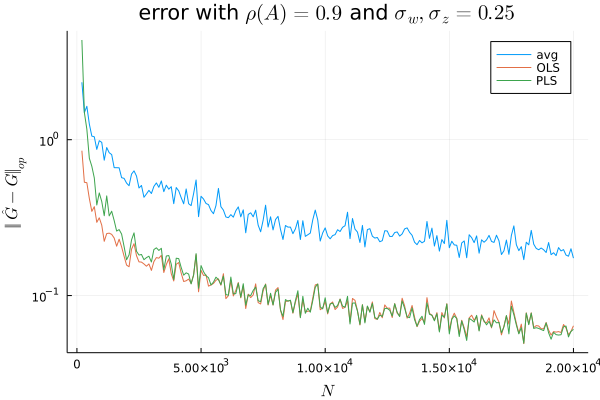
\includegraphics[scale=0.6]{rho_small}
\end{figure}
\end{frame}

\begin{frame}
\begin{figure}
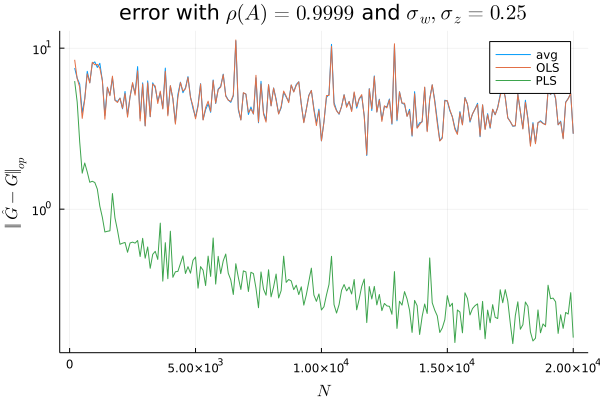
\includegraphics[scale=0.6]{rho_1me}
\end{figure}
\end{frame}

\begin{frame}
\begin{figure}
\includegraphics[scale=0.6]{baseline_stability}
\end{figure}
\end{frame}
